\documentclass{article}


\usepackage[]{geometry}

\usepackage{titling} % center cover page
\renewcommand\maketitlehooka{\null\vfill} % center cover page
\renewcommand\maketitlehookd{\vfill\null} % center cover page

\usepackage{tocloft} % add dots for sections in table of contents
\renewcommand{\cftsecleader}{\cftdotfill{\cftdotsep}} % add dots for sections in table of contents

\usepackage{hyperref} % make table of contents clickable
\hypersetup{ % remove default ugly look of links
	colorlinks,
	citecolor=black,
	filecolor=black,
	linkcolor=black,
	urlcolor=black
}

%\AddToHook{cmd/section/before}{\clearpage} % each section starts on new page

\usepackage{acronym} % acronyms

\usepackage{graphicx} % required to load images
\graphicspath{ {./source-items/imgs/} }

\usepackage{listings} % to format SQL code

\usepackage{color} % to format SQL code

\definecolor{dkgreen}{rgb}{0,0.6,0}
\definecolor{gray}{rgb}{0.5,0.5,0.5}
\definecolor{mauve}{rgb}{0.58,0,0.82}

\lstset{language=SQL,	% to format SQL code
	basicstyle={\small\ttfamily},
	belowskip=3mm,
	breakatwhitespace=true,
	breaklines=true,
	classoffset=0,
	columns=flexible,
	commentstyle=\color{dkgreen},
	framexleftmargin=0.25em,
	frameshape={}{}{}{},	% to add to vertical lines on left, set `frameshape={}{YY}{}{}`
	keywordstyle=\color{blue},
%	numbers=left,	% if you want line numbers, set `numbers=left`
%	numberstyle=\tiny\color{gray},
	showstringspaces=false,
	stringstyle=\color{mauve},
	tabsize=3,
	xleftmargin =1em,
	escapeinside={(@*}{*@)}
}

\lstdefinestyle{DOS}	% to format cmd code
{
	backgroundcolor=\color{black},
	basicstyle=\scriptsize\color{white}\ttfamily
}

\usepackage{subfig}

\usepackage{float}



\hypersetup{pdftitle={Databases - RDBMS - SQL - English}}
\hypersetup{pdfauthor={Spyros Alertas}}
\hypersetup{pdfsubject={Databases - RDBMS - SQL - Notes}}
\hypersetup{pdfkeywords={Databases, Relational Databases, Relational Database Management Systems, DBMS, RDBMS, SQL, MySQL}}

\title{\bfseries{Databases - RDBMS - SQL}}

\author{Spyros Alertas}

\date{Created On: July 24, 2023\\Last Edit: \today}

% Hint: \title{whatever}, \author{who cares} and \date{whenever} could stand before or after the \begin{document} command BUT the \maketitle command MUST come AFTER the \begin{document} command!

\begin{document}


% cover page
\begin{titlingpage}
\maketitle
\end{titlingpage}


% table of contents
\tableofcontents


% all sections - main document content

\newpage
\section{Introduction}
\paragraph{} In this document I try to cover a vast content of concepts of
\aclp{DB}, some more basic and useful to any role while others are more advanced. I tried to write the content in a linear to follow way so that even with little experience one can follow to learn.
\paragraph{} \acs{SQL} commands are tested using My\acs{SQL} version 8. If you are using different Major version or different \acs{DBMS}, commands might slightly differ in some cases, however the concepts should be the same. In most cases I try to provide the equivalent commands for Oracle \acs{SQL} as well (tested on version 12c).



\section{\acl{DB}, \acs{DBMS} and \acs{RDBMS} Definitions}
\label{sec:db}
\paragraph{} \textbf{\acl{DB}} is an organized collection of related data.
\label{sec:dbms}
\paragraph{} \textbf{\acf{DBMS}} is the interface that allows us to access and manipulate the data in the \acl{DB}.
\label{sec:rdbms}
\paragraph{} \textbf{\acf{RDBMS}} is a \acs{DBMS} used for Relational \aclp{DB}.
\begin{center}
	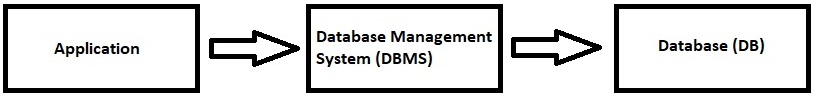
\includegraphics[scale=0.8]{app-dbms-db-flow}
\end{center}


\section{Theory of Relational \aclp{DB}}
\paragraph{} Brief description of basic terminology of Relational \aclp{DB}.
\begin{itemize}
	\item \textbf{Relational \acs{DB}} is a way of structuring information in tables, rows and columns with the ability to create relationships between the tables and their data.
	\item \textbf{Table} is a collection of related data stored in a table format within the database; consisting of rows and columns.
	\item \textbf{Row} or \textbf{Tuple} is a single, implicitly structured data item in a table. Every row in the table has the same structure.
	\item \textbf{Column} is a set of data values of a particular type that will hold the value for a specific information for each row.
	\item \textbf{\acl{P.K.}} is a column or a set of columns that uniquely identify each row in the table. Each table can have only one \acl{P.K.}.
	\item \textbf{\acl {F.K.}} is used to establish relationships between two entities. The \acl {F.K.} of one table is the \acl{P.K.} of another table. In some cases the \acl {F.K.} might reference the \acl{P.K.} of the same table it exists in.
\end{itemize}
\paragraph{} Small practical example of above definitions for better understanding.
\begin{figure}[h]
	\centering
	\subfloat[\centering Table: BOOK]{{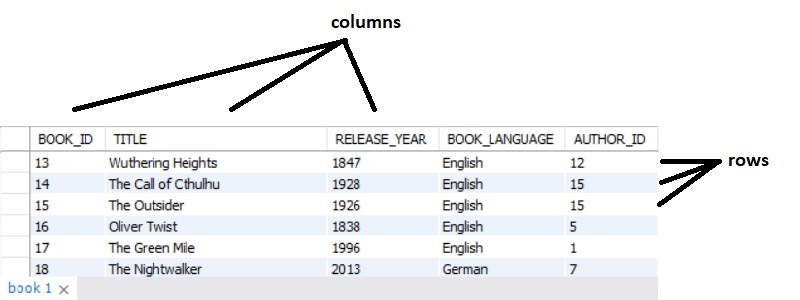
\includegraphics[width=5cm]{books-01}}}
	\qquad
	\subfloat[\centering Table: AUTHOR]{{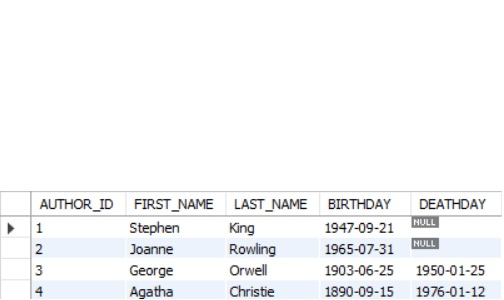
\includegraphics[width=5cm]{authors-01}}}
\end{figure}
\paragraph{} In this example in above images we have:
\begin{itemize}
	\item \textbf{Tables}: BOOK (a) and AUTHOR (b).
	\item \textbf{Rows} 6 in table BOOK and 4 in table AUTHOR. Example row: 16, Oliver Twist, 1838, English, 5.
	\item \textbf{Columns} 5 in table BOOK and 5 in table AUTHOR. Example column title in table BOOK.
	\item \textbf{\acl{P.K.}} is book\_id for table BOOK and author\_id for table AUTHOR.
	\item \textbf{\acl{F.K.}} is author\_id in table BOOK and defines which is the author for each book.
\end{itemize}


\section{Table Relationships}
\paragraph{} There are three types of tables relationships.
\begin{enumerate}
	\item \textbf{One to One:} For each record in the primary table, there can be only one record in the foreign table. It can be achieved by using the primary key of the foreign table as foreign key with unique constraint.
	\item \textbf{One to Many:} For each record in the primary table, there can be many records in the foreign table, but for each record in the foreign table, there can be only one record in the primary table. It can be achieved by using the primary key of the foreign table as foreign key.
	\item \textbf{Many to Many:} For each record in the primary table, there can be many records in the foreign table, but also for the foreign table there can be many records in the primary table. It can be achieved by using a third table, that will consist of the primary keys of the two tables.
\end{enumerate}


\section{\acf{SQL} and My\acs{SQL}}
\label{sec:sql}
\paragraph{} \textbf{\acf{SQL}} is the language used to communicate with the \acl{DB}. \acs{SQL} is a standard that all \acsp{RDBMS} need to implement.
\label{sec:mysql}
\paragraph{} \textbf{My\acs{SQL}} is one of the most popular implementations of \acs{SQL}.
\label{sec:listofrdbms}
\paragraph{} \textbf{Some of the most important and popular \acsp{RDBMS}:}
\begin{itemize}
	\item\href{https://en.wikipedia.org/wiki/MySQL}{My\acs{SQL} - Wikipedia}
	\item\href{https://en.wikipedia.org/wiki/Oracle_Database}{Oracle Database - Wikipedia}
	\item\href{https://en.wikipedia.org/wiki/Microsoft_SQL_Server}{Microsoft \acs{SQL} Server - Wikipedia}
	\item\href{https://en.wikipedia.org/wiki/PostgreSQL}{Postgre\acs{SQL} - Wikipedia}
	\item\href{https://en.wikipedia.org/wiki/SQLite}{\acs{SQL}ite - Wikipedia}
\end{itemize}

\section{Types of SQL Commands}
\paragraph{} There are five different sub-languages \acs{SQL}: \acs{DCL}, \acs{DDL}, \acs{DML}, \acs{DQL} and \acs{TCL}.
\begin{center}
	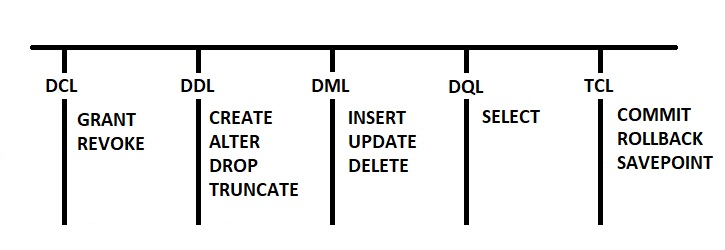
\includegraphics[scale=0.8]{types-of-sql-commands}
\end{center}
\paragraph{} \textbf{\acf{DCL}}
\begin{itemize}
	\item Is responsible for administrative tasks, mainly granting and revoking user privileges.
	\item \textbf{\acs{DCL} commands:}
	\subitem GRANT/REVOKE/FLUSH PRIVILEGES, SHOW GRANTS.
	\item \textbf{Non \acs{DCL} commands} covered in this section as they are related to \acs{DB} users and roles:
	\subitem CREATE/RENAME/DROP USER.
	\subitem CREATE/RENAME/DROP/SET DEFAULT ROLE.
\end{itemize}
\paragraph{} \textbf{\acf{DDL}}
\begin{itemize}
	\item Is responsible for defining the structure of the data.
	\item \textbf{Important:} \acs{DDL} commands are auto-committed, once executed changes are permanently saved in the database. Rollback is not possible.
	\item \textbf{\acs{DDL} commands:}
	\subitem CREATE/ALTER/DROP/TRUNCATE/COMMENT/RENAME TABLE.
	\subitem CREATE/DROP VIEW.
	\subitem CREATE/DROP/SHOW/USE DATABASE.
\end{itemize}
\paragraph{} \textbf{\acf{DML}}
\begin{itemize}
	\item Is responsible for creating, updating and deleting data.
	\item From \acs{CRUD} operations it is responsible for: Create, Update and Delete operations.
	\item \textbf{\acs{DML} commands:}
	\subitem INSERT/UPDATE/MERGE/DELETE.
\end{itemize}
\paragraph{} \textbf{\acf{DQL}}
\begin{itemize}
	\item Is responsible for reading/querying data from the database.
	\item From \acs{CRUD} operations it is responsible for: Read operation.
	\item \textbf{\acs{DQL} commands:}
	\subitem SELECT.
\end{itemize}
\paragraph{} \textbf{\acf{TCL}}
\begin{itemize}
	\item Is responsible for controlling transaction behavior.
	\item \acs{TCL} commands $\underline{can}$ only be used with \acs{DML} and \acs{DQL} commands.
	\item \acs{TCL} commands $\underline{cannot}$ be used with \acs{DCL} or \acs{DDL} commands as they are auto-committed.
	\item \textbf{\acs{TCL} commands:}
	\subitem START TRANSACTION/COMMIT/ROLLBACK.
	\subitem SAVEPOINT/ROLLBACK TO SAVEPOINT.
	\subitem START TRANSACTION READ WRITE/READ ONLY.
	\subitem SET TRANSACTION ISOLATION LEVEL.
	\subsubitem SERIALIZABLE/READ COMMITTED/UNCOMMITTED/REPEATABLE.
\end{itemize}

\section{Setup MySQL}
\paragraph{} Download MySQL Installer (version 8+) from \href{https://dev.mysql.com/downloads/installer/}{here}. During installation make sure to select for install the following components: MySQL Server, MySQL Workbench. And these: Connector/J, MySQL Documentation, Samples and Examples, MySQL Shell.
\paragraph{} When MySQL installation is finished, open MySQL Workbench, in the middle of the screen, next to MySQL Connections, click on the + icon. There put any connection name you want, the username and the password you created for root and admin accounts during installation. The other fields we will leave with their default values for now.


\section{\acs{DCL} Commands In Depth}
\paragraph{} In this section we will cover the \acf{DCL} commands and everything related to user and role management.\\\textbf{Purpose:} deal with the rights and permissions of the users on the database.\\\textbf{Users:} are user accounts that can connect in the \acs{DB} to perform their tasks.\\\textbf{Roles:} are like predefined sets of privileges that can be granted to users.\\Connect with MySQL Workbench as root or admin user to execute the following commands.\\\textbf{Auto-Commit:} Yes. Once a \acs{DCL} command is executed changes will be permanent, no rollback option.
\subsection{User Management}
\paragraph{} \textbf{Note:} These are not \acs{DCL} commands but we need them to see the content in a linear way. These commands are all auto-committed, once executed changes are saved in \acs{DB} without the ability to do rollback.
\begin{lstlisting}[language=SQL]
	-- Create new user
	-- Syntax: create user '<username>'@'<hostname>' identified by '<password>';
	-- Example:
	create user 'testuser'@'localhost' identified by 'testpass';
	-- Note: By default new users have no privileges. They have to be granted their privileges seperately.
	
	-- View current users
	-- MySQL Syntax:
	select * from mysql.user;
	
	-- Rename user
	-- Syntax: rename user '<oldusername>'@'<hostname>' to '<newusername>'@'<hostname>';
	-- Example:
	rename user 'testuser'@'localhost' to 'realuser'@'localhost';
	
	-- Delete user
	-- Syntax: drop user '<username>'@'<hostname>';
	-- Example:
	drop user 'realuser'@'localhost';
\end{lstlisting}
\subsection{Grant/Revoke Privileges}
\begin{lstlisting}[language=SQL]
	-- View admin level privileges of users (like create/drop databases, users etc)
	-- NySQL Syntax:
	select * from mysql.user;
	
	-- Create testuser to experiment with
	create user 'testuser'@'localhost' identified by 'testpass';
	-- create testdb to expirement with
	create database testdb;
	
	-- See user privileges on databasese and tables
	-- Syntax: show grants for '<username>'@'<hostname>';
	-- Example:
	show grants for 'admin'@'%';
	show grants for 'testuser'@'localhost';
	
	-- View list of all available privileges
	show privileges;
	
	-- Alter user privileges
	-- Give all permissions for specific database
	-- Syntax: grant all privileges on <db_name>.* TO '<username>'@'<hostname>';
	-- Example
	grant all privileges on testdb.* TO 'testuser'@'localhost';
	-- * can be replaced with table name, in that case privileges will be granted on table level and not on db
	
	-- Remove all permissions for specific database
	-- Syntax: revoke all privileges on <db_name>.* from '<username>'@'<hostname>';
	-- Example:
	revoke all privileges on testdb.* from 'testuser'@'localhost';
	
	-- Give specific permission(s) only 
	-- Syntax: grant <privilegeA>, <privilegeB>, <....> on <db_name>.* to '<username>'@'<hostname>';
	-- Example - Give only insert, select permissions on all tables for DB:
	grant insert, select on testdb.* to 'testuser'@'localhost';
	
	-- Remove specific permission(s) only
	-- Syntax: revoke <privilegeA>, <privilegeB>, <....> on <db_name>.* from '<username>'@'<hostname>';
	-- Example - Revoke only INSERT permission from user:
	revoke insert on testdb.* from 'testuser'@'localhost';
	
	-- Flush privileges is required to make the changes effective, only when we
	-- directly modify the privileges in the grant tables using insert, update, delete.
	-- Syntax:
	flush privileges;
	
	-- Note: Privilege changes may not be reflected on existing DB sessions.
\end{lstlisting}
\subsection{Role Management}
\paragraph{} The purpose of roles is to easily grant specific set of privileges to users based on the role we want them to have on the database.
\begin{lstlisting}[language=SQL]
	-- Create new role
	-- Syntax: create role <rolename>;
	-- Example:
	create role 'testrole';
	
	-- View existing roles in DB
	-- MySQL Syntax:
	select * from mysql.user where authentication_string = ''; -- only roles should have empty authentication string
	
	-- Rename Role:
	-- Syntax: rename user <oldrolename> to <newrolename>;
	-- Example:
	rename user 'testrole' to 'mytestrole';
	
	-- Add privileges to role
	-- Syntax: grant all privileges on <db_name>.* to 'role';
	-- Example:
	grant all privileges on testdb.* to 'mytestrole';
	
	-- Remove privileges from role
	-- Syntax: revoke all privileges on <db_name>.* from 'role';
	-- Example:
	revoke all privileges on testdb.* from 'mytestrole';
	
	show grants for 'mytestrole';
	
	-- Add role to user
	-- Syntax: grant <role> to '<user>'@'<host>';
	-- Example:
	grant 'mytestrole' to 'testuser'@'localhost';
	
	-- Remove role from user
	-- Syntax: revoke <role> from '<user>'@'<host>';
	-- Example:
	revoke 'mytestrole' from 'testuser'@'localhost';
	
	show grants for 'testuser'@'localhost';
	
	-- Set default role for user
	-- Syntax: set default role '<role>' to '<user>'@'<host>';
	-- Example:
	set default role 'mytestrole' to 'testuser'@'localhost';
	
	-- Remove default role from user
	-- Syntax: set default role none to '<user>'@'<host>';
	-- Example:
	set default role none to 'testuser'@'localhost';
	
	-- View current users role
	-- Syntax:
	select current_role();
	
	-- Delete role
	-- Syntax: drop role <rolename>;
	-- Example:
	drop role 'mytestrole';
	
	drop user 'testuser'@'localhost';
	drop database testdb;
\end{lstlisting}
\subsection{Initialize Sample Database}
\paragraph{} At this point please run these two scripts below as admin to create the database and insert sample data.\\
1-SQL Script to create tables: \href{file:./source-items/sql/books-db-init/booksdb-create-tables.sql}{click here}.\\
2-SQL Script to insert data: \href{file:./source-items/sql/books-db-init/booksdb-insert-data.sql}{click here}.
\subsection{Practice: Role and User Management}
\begin{lstlisting}[language=SQL]
	select * from mysql.user;
	
	create user 'bookso'@'localhost' identified by 'bookso';
	show grants for 'bookso'@'localhost';
	
	-- Open another session (let's name it session B) as bookso user now and run
	show databases; -- database booksdb won't be visible
	
	grant all privileges on booksdb.* to 'bookso'@'localhost';
	
	-- On Session B as bookso user run again
	show databases; -- database booksdb will be visible and with grant all we are able to do any operation on the db
	
	revoke all privileges on booksdb.* from 'bookso'@'localhost';
	
	create role 'books_read_role';
	create role 'books_insert_role';
	create role 'books_delete_role';
	
	select * from mysql.user where authentication_string = '';
	
	show grants for 'books_read_role';
	grant select on booksdb.* to 'books_read_role';
	
	show grants for 'books_insert_role';
	grant insert on booksdb.* to 'books_insert_role';
	
	show grants for 'books_delete_role';
	grant delete on booksdb.* to 'books_delete_role';
	
	grant 'books_read_role' to 'bookso'@'localhost';
	grant 'books_insert_role' to 'bookso'@'localhost';
	grant 'books_delete_role' to 'bookso'@'localhost';
	show grants for 'bookso'@'localhost';
	
	-- Note: By default roles are not active on users, this means users won't have these privileges
	-- even if they are granted these privileges.
	
	-- Open a new session as a bookso user and run below commands
	show databases; -- booksdb database won't be visible
	-- Solution 1 (Per Session Only):
	select current_role(); -- will be none
	set role 'books_read_role'; -- after this command above command will show new role
	-- You can also asign a list of roles:
	set role 'books_read_role', 'books_insert_role';
	
	-- This way the user has the privileges of the set roles only.
	-- With set role, each time you open a new session you will have to set again each role.
	
	-- Solution 2 (Permanent):
	set default role 'books_insert_role', 'books_read_role' to 'bookso'@'localhost';
	
	-- Now open a new session as bookso and run below command, all above roles will be listed
	select current_role(); -- will show all 3 above roles
	
	-- Note: If you set the role for the user of current user the part to 'user'@'host' is optional
	-- but if you set it for another user it's mandatory
	
	-- Note: Such changes won't be reflected to existing sessions, only on new ones (set default role)
	
	-- Clean up
	drop role 'books_insert_role', 'books_read_role', 'books_delete_role';
	grant all privileges on booksdb.* to 'bookso'@'localhost';
\end{lstlisting}
\subsection{Section Notes}
\begin{itemize}
	\item For all \acs{SQL}/\acs{DCL} commands of this section \href{file:./source-items/sql/1-sql-dcl.sql}{click here}.
	\item For more on account management statements \href{https://dev.mysql.com/doc/refman/8.0/en/account-management-statements.html}{click here}.
\end{itemize}


\section{\acs{DDL} Commands In Depth}
\paragraph{} In this section we will cover the \acf{DDL} commands. These commands deal with the structure of the database itself, like create tables, views, procedures etc. or modify/delete them.\\\textbf{Purpose:} Define the structure of the database and its objects.\\\textbf{Auto-Commit:} Yes. Once a \acs{DDL} command is executed changes will be permanent, no rollback option.
\subsection{Schema Management}
\paragraph{} Schema is a collection of database objects, like tables, views, triggers, etc.
\begin{lstlisting}[language=SQL]
	-- Create a database schema
	-- Syntax: create database <schema_name>;
	-- Example:
	create database customer;
	
	-- View list of all existing schemas (current user has access to)
	show databases;
	
	-- View currently active/in use schema
	select database();
	
	-- select active schema for use
	-- Syntax: use <schema_name>;
	-- Example:
	use customer;
	
	-- Delete database schema
	-- Syntax: drop database <schema_name>;
	-- Example:
	drop database customer;
\end{lstlisting}
\subsection{Table Management}
\paragraph{} Table is the base component of relational databases, it's the place that data are stored based on the defined structure.
\begin{lstlisting}[language=SQL]
	use booksdb;
	select database();
	show tables;
	
	-- Create new table
	-- Syntax: create table <table_name> (column1 datatype, column2 datatype, column3 datatype ....);
	-- Example:
	create table customer (
	customer_id bigint primary key auto_increment,
	first_name varchar(50) not null,
	last_name varchar(50),
	birthdate date,
	age int,
	constraint is_adult_failed check (age > 18)
	);
	create table products (
	product_id bigint auto_increment,
	pname varchar(10) not null,
	pstatus char(1) default 'E',
	customer_id bigint,
	primary key (product_id),
	foreign key (customer_id) references customer (customer_id)
	);
	-- Some notes:
	-- 1. Table product references table customer, so customer has to be created first.
	-- 2. In the two tables we see the two different ways of defining the primary key; the primary key may consist of more than one column.
	-- 3. Primary keys cannot be null.
	-- 4. not null vs default: not null means during insert/update you have to give any non null valid value for that column. Default means, if no value is passed during insert for that column, default value will be used. However during insert or update, null is a valid value to set for the column.
	-- 5. char vs varchar: char means fixed size in storage, if we set char(10) for example, even if we give as value the string 'Hi', the space used in storage will be for 10 chars. With varchar(10) however the size is not fixed, depending on the size of the string, the required space will be used. In both cases, string longer than the given value will cause failure or data to be truncated.
	-- 6. We can add check constraints named or unnamed to prevent invalid data from being inserted in the database.
	-- 7. Foreign key can be null, if we don't explicitly say not null, however if value is given, that value must exist in the reference table.
	-- 8. auto_increment means if no value is passed, it will take the max value of that table column + 1.
\end{lstlisting}
\begin{itemize}
	\item For more on create tables \href{https://dev.mysql.com/doc/refman/8.0/en/create-table.html}{click here}.
	\item For more on data types \href{https://dev.mysql.com/doc/refman/8.0/en/data-types.html}{click here}.
\end{itemize}
\subsection{Practice: Understand Created Tables}
\paragraph{} The commands in this section are not \acs{DDL}, they are \acs{DML} and \acs{DQL}, just to see in practice how primary keys, foreign keys, check constraints etc work to get a better understanding.
\begin{lstlisting}[language=SQL]
	-- Tables are initially empty
	select * from customer;
	select * from products;
	
	-- customer table
	insert into customer 
	(customer_id, first_name, last_name, birthdate, age)
	values
	(1, 'Spyros', null, null, null)
	; -- will work
	insert into customer 
	(customer_id, first_name, last_name, birthdate, age)
	values
	(2, 'John', 'Wick', null, 15)
	; -- will fail due to age constraint validation
	insert into customer 
	(customer_id, first_name, last_name, birthdate, age)
	values
	(2, 'John', 'Wick', null, 45)
	; -- will work
	insert into customer 
	(first_name, last_name, birthdate, age)
	values
	('Bruce', 'Willis', null, 45)
	; -- will work (we removed customer id but will be auto populated due to auto_increment attribute)
	insert into customer 
	(customer_id, first_name, last_name, birthdate, age)
	values
	(3, 'Nick', null, null, 45)
	; -- will fail due to duplicate primary key
	select * from customer;
	
	-- products table
	insert into products
	(product_id, pname, pstatus, customer_id)
	values
	(3, 'R7', null, 4)
	; -- will fail because we gave inexistent foreign key
	insert into products
	(product_id, pname, pstatus, customer_id)
	values
	(2, 'Ryzen 7 1700', null, 1)
	; -- will fail because data is too long for column pname
	insert into products
	(product_id, pname, pstatus, customer_id)
	values
	(3, 'R7 ', null, 1)
	; -- will work
	insert into products
	(product_id, pname, pstatus, customer_id)
	values
	(5, 'R8 ', 'D', 3)
	; -- will work
	insert into products
	(pname, customer_id)
	values
	('R9 ', 2)
	; -- will work
	
	delete from customer where customer_id = '1'; -- will fail because there are data in table products that reference that customer id
	
	select * from customer;
	select * from products;
\end{lstlisting}
\subsection{More on Table Management}
\begin{lstlisting}[language=SQL]
	-- Create table with select from another table - using where clause we can only keep data that satisfy certain conditions
	-- Syntax: create table <backup_table_name> select * from <original_table_name>;
	-- Example:
	create table customer_backup_26082023 select * from customer;
	
	select * from customer_backup_26082023;
	
	-- Create table with same structure of another table but without data
	-- Syntax: create table <clone_table_name> select * from <original_table_name> where 1 = 2;
	-- Example:
	create table products_clone select * from products where 1 = 2; -- 1 = 2 will never be true and is used to insert no data
	
	select * from products_clone; -- no data
	
	desc products;
	desc products_clone; -- notice that PK/FK/auto_increment/check constraints etc are not copied on the new table, only the structure.
	
	-- Rename table
	-- Syntax: rename table <original_table_name> to <new_table_name>;
	-- Example:
	rename table products to product;
	
	select * from products; -- no table with name products now
	select * from product;
	
	-- Alternatively alter can be used
	-- Syntax: alter table <original_table_name> to <new_table_name>;
	-- Example:
	alter table products_clone rename products_clone2;
	
	select * from products_clone; -- no table with this name now
	select * from products_clone2;
	
	-- Alter table
	-- Alter table can be used to modify the attributes of existing tables, viewe or any database object
	-- Depending on the DBMS and its settings, what is allowed and what is not allowed to alter might slightly differ
	
	-- Remove column from table
	-- Syntax: alter table <table_name> drop <column_name>;
	alter table customer drop age;
	-- confirm column is removed
	desc customer;
	-- Add column to table
	-- Syntax: alter table <table_name> add <column_name>;
	alter table customer add age int constraint is_adult_failed check (age > 18);
	-- confirm column is added back
	desc customer;
	
	-- Truncate table
	-- Truncate drops and creates again the table but without data
	select * from customer_backup_26082023; -- table has data before truncate
	
	-- Syntax: truncate <table_name>;
	-- Example:
	truncate customer_backup_26082023;
	
	select * from customer_backup_26082023; -- no data after truncate but table still exists
	
	-- Alternatively - However this is wrong way to delete all data from a table
	-- Syntax: delete from <table_name>;
	delete from customer_backup_26082023; -- without where clause it will delete all data from the table
	
	-- View table details
	-- Syntax A: describe <table_name>;
	-- Syntax B: desc <table_name>;
	-- Example:
	desc customer;
	
	-- Drop table
	-- Syntax: drop table <table_name>;
	-- Example:
	drop table customer_backup_26082023;
	drop table products_clone2;
	
	-- Truncate vs Delete vs Drop
	-- Truncate: Truncate is used to delete all the data from a table but keep the table itself.
	-- Truncate will drop and create again the table.
	-- Delete: without where clause will also empty the table. However because delete will have to go through the whole
	-- table and delete each row individually, which is a lot slower and resource intensive than truncate.
	-- Drop: Completely deletes the table and all its data.
	
	-- Clean-up DB
	drop table product;
	drop table customer;
\end{lstlisting}
\begin{itemize}
	\item Fore more on alter tables \href{https://dev.mysql.com/doc/refman/8.0/en/alter-table.html}{click here}.
\end{itemize}
\subsection{Views}
\paragraph{} Views act like virtual tables to give as an opinionated view of the data. Depending on how the view is created it may or may not allow insert/update/delete operations. However if these operations are allowed, the changes will be done on the actual tables and not only on the view.
\begin{lstlisting}[language=SQL]
	select	c.customer_id, c.first_name, c.last_name, p.product_id, p.pname, p.pstatus
	from	customer as c, product as p
	where	c.customer_id = p.customer_id;
	-- With above query we get all customers and their products and with specified columns
	-- Products without customer (if any exist) won't be in the result set
	
	-- Create view
	-- Syntax: create view <viewname> as select <columnnameA>, <columnnameB>, .... from <tablenamea>, <tablenameb>, .... WHERE <conditions>;
	-- Example:
	create view customer_products as
	select	c.customer_id, c.first_name, c.last_name, p.product_id, p.pname, p.pstatus
	from	customer as c, product as p
	where	c.customer_id = p.customer_id
	;
	
	-- Now instead of previous big query we can just do:
	select * from customer_products; -- and get same results
	
	-- Update view
	-- Syntax: create or replace view <viewname> as select <columnnameA>, <columnnameB>, .... from <tablenamea>, <tablenameb>, .... WHERE <conditions>;
	-- Example:
	create or replace view customer_products as
	select	c.customer_id, c.first_name, c.last_name, c.age, p.product_id, p.pname, p.pstatus
	from	customer as c, product as p
	where	c.customer_id = p.customer_id
	;
	-- create or replace, if view exists it will change it (if there is anything different) or create it if it doesn't exist
	
	desc customer_products;
	
	-- Drop view
	-- Syntax: drop view <viewname>;
	-- Example:
	drop view customer_products;
	
	-- Clean-up DB
	drop table product;
	drop table customer;
\end{lstlisting}
\begin{itemize}
	\item Fore more on views \href{https://dev.mysql.com/doc/refman/8.0/en/views.html}{click here}.
	\item Fore more on updatable/insertable views \href{https://dev.mysql.com/doc/refman/8.0/en/view-updatability.html}{click here}.
\end{itemize}
\subsection{Section Notes}
\begin{itemize}
	\item For all \acs{SQL}/\acs{DDL} commands of this section \href{file:./source-items/sql/2-sql-ddl.sql}{click here}.
\end{itemize}


\section{\acs{DML} Commands In Depth}
\paragraph{} In this section we will cover the \acf{DML} commands which allow us to modify the data in the database. From \acs{CRUD}, these commands are responsible for Create/Update/Delete operations.\\\textbf{Purpose:} Modify data in the database.\\\textbf{Auto-Commit:} No. Some \acs{DBMS} auto-commit \acs{DML} commands as well.
\subsection{Preparation}
\begin{lstlisting}[language=SQL]
	-- Note: Insert/Update/Delete are DDL commands; start transaction/commit/rollback are TCL commands
	
	-- Note: In MySQL by default only safe update/delete is allowed, which means only by using a primary key in where clause. To change this please run below two commands:
	set global sql_safe_updates = 0; -- disable safe updates for all sessions
	set sql_safe_updates = 0; -- disable safe updates for current session only
	
	show global variables like 'sql_safe_updates';
	show variables like 'sql_safe_updates';
	
	-- This global variable is ignored in MySQL Workbench unless you change below setting:
	-- MySQL Workbench -> Edit -> Preferences -> SQL Editor -> Uncheck Safe Updates box at the end
	
	-- Note: In MySQL even DML commands are autocommited. There are two methods to work around this:
	-- Method 1: Disable auto-commit variable to 0
	set global autocommit = 0; -- disable autocommit for all sessions
	set autocommit = 0; -- disable autocommit for current session only
	
	show global variables like 'autocommit';
	show variables like 'autocommit';
	
	-- This global variable is also ignored unless you change below setting:
	-- MySQL Workbench -> Edit -> Preferences -> SQL Execution -> Uncheck New connections use auto commit mode
	
	-- Method 2: Start a transaction before executing DML commands
	start transaction;
	-- run DML commands - changes won't saved untill you commit or rollback
	commit;
	-- or
	rollback;
	-- to complete the transaction by saving or reverting the changes
	
	-- Note: If you commit or rollback, then you have to start another transaction, else DML commands will auto-commit again
	-- Note: Each time start transaction; is executed, pending changes in current session will be committed
\end{lstlisting}
\subsection{Insert}
\begin{lstlisting}[language=SQL]
	use booksdb;
	
	desc book;
	
	-- Insert
	-- Syntax: insert into <table_name>
	-- Example:
	start transaction;
	insert into book
	(title, release_year, book_language)
	values
	('New Experimental Cook Book', 2004, 'English')
	;
	commit;
	rollback; -- if you rollback before commit, change will be lost, if you rollback after commit, change is permanent already
	select * from book where title = 'New Experimental Cook Book';
	
	-- If you give all values in same order as they appear in table, syntax can change as below (skipping column names)
	-- Syntax:
	-- insert into book (value1, value2, ....);
	
	-- Insert using select (can also be from different table)
	-- Syntax: insert into <table_name> <columnA, columnB, .... > select <columnA, columnB> from <table_name> where <conditions>;
	-- Example:
	start transaction;
	insert into book
	(title, release_year, book_language)
	select 'Animal Farm v2', release_year + 5, book_language
	from book
	where title = 'Animal Farm'
	;
	commit;
	select * from book where title = 'Animal Farm';
	select * from book where title = 'Animal Farm v2';
\end{lstlisting}
\subsection{Update}
\begin{lstlisting}[language=SQL]
	-- Hint: Before update it's always a good idea to run a select query, to check what the where clause will return. If the were clause is not correct, undesired rows may be updated, if you do select first you can confirm it works as should. Same advice goes for delete.
	
	select * from book where title = 'New Experimental Cook Book'; -- 1 row
	
	-- Update
	-- Syntax: update <table_name> set <columnA = 'valueA', columnB = 'valueB', ....> where <conditions>;
	-- Example:
	start transaction;
	update book
	set release_year = 2006
	where title = 'New Experimental Cook Book'; -- 1 row updated
	commit; -- if more than expected rows are updated rollback and check
\end{lstlisting}
\subsection{Delete}
\begin{lstlisting}[language=SQL]
	select * from book where title = 'Animal Farm v2'; -- 1 row
	select * from book where title = 'New Experimental Cook Book'; -- 1 row
	
	-- Syntax: delete from <table_name> where <conditions>;
	-- Example:
	start transaction;
	delete from book
	where title = 'New Experimental Cook Book'; -- 1 row deleted
	delete from book
	w`here title = 'Animal Farm v2'; -- 1 row deleted
	commit;
\end{lstlisting}
\subsection{Section Notes}
\begin{itemize}
	\item For more on insert \href{https://dev.mysql.com/doc/refman/8.0/en/insert.html}{click here}.
	\item For more on update \href{https://dev.mysql.com/doc/refman/8.0/en/update.html}{click here}.
	\item For more on delete \href{https://dev.mysql.com/doc/refman/8.0/en/delete.html}{click here}.
	\item For all \acs{SQL}/\acs{DML} commands of this section \href{file:./source-items/sql/3-sql-dml.sql}{click here}.
\end{itemize}


\section{\acs{DQL} Commands In Depth}
\paragraph{} In this section we will cover the \acf{DQL} commands. The select statement is also called query, because it's responsible for querying the database to read data from it. What we will see here can be applied also to \acs{DML} commands.\\\textbf{Purpose:} Define the structure of the database and its objects.\\\textbf{Auto-Commit:} No.
\subsection{Basic DQL Operations}
\begin{lstlisting}[language=SQL]
-- Content Summary:
-- Single Quotes ' vs Double Quotes "
-- Equal/Not Equal/Greater/Greater or Equal/Less/Less or Equal
-- In/Not In/Is Null/Is Not Null/Like/Not Like/Wildcards/Escape Wildcards and Special Characters
-- And/Or and ()
-- Between/Not Between/Order By (Asc/Desc)
-- Alias
-- Distinct
-- Show Warnings

-- Single Quotes ' vs Double Quotes "
-- The standard supported in all SQL Systems is Single Quotes to define Strings
-- Double Quotes are supported by some DBMS but it's not a standard
select * from book where book_title = 'IT'; -- Standard SQL, supported by all DBMS
select * from book where book_title = "IT"; -- Non Standard SQL, may not work in some DBMS

-- Equal: =
select * from book where book_language = 'Italian';
-- Not Equal: <>
select * from book where book_language <> 'English';

-- Greater: >
select * from book where release_year > 2009;
-- Greater or Equal: >=
select * from book where release_year >= 2009;
-- Less: <
select * from book where release_year < 1521;
-- Less or Equal: <=
select * from book where release_year <= 1521;

-- In: in (value1, value2, ....)
select * from book where book_language in ('German', 'French');
-- Not In: not in (value1, value2, ....)
select * from book where book_language not in ('English', 'German');

-- Is Null: is null (= null is not working)
select * from author where deathday is null;
-- Is Not Null: is not null (<> null is not working)
select * from author where deathday is not null;

-- Like:
select * from author where first_name like 'Da%'; -- match 0 or any number of any characters
select * from author where first_name like 'Da_'; -- match exactly one any character
-- Not Like:
select * from author where first_name not like 'D%';

-- Wildcards:
-- %: match with 0 or any number of any character
-- _: match with exactly one any character
-- wildcards act as wildcards only with like/not like, not with = or <>

-- Escape wildcards/Special Characters:
select * from book where title like '%Handmaid\'s%';
-- Use \ before any wildcard/special character if you want sql to treat it as normal character

-- And/Or
select * from author where first_name like 'Da%' and first_name not like 'Da_';
select * from author where first_name like 'Da%' or first_name like 'Sa%';

-- Use of () to specify the priority of logical operations with and/or
-- If no () is used, SQL will apply the conditions from left to write

-- Example:
select * from author where (first_name like 'Da%' or first_name like 'Sa%') and birthday like '19%'; -- 2 rows
select * from author where first_name like 'Da%' or first_name like 'Sa%' and birthday like '19%'; -- 3 rows
-- why second query gives one more row? because SQL executes the operations from left to write so it's equivalent to below
select * from author where first_name like 'Da%' or (first_name like 'Sa%' and birthday like '19%'); -- 3 rows
-- so the condition and birthday like '19%' is applied only for names that start with Sa

-- Between
select * from book where release_year >= 1950 and release_year <= 1955; -- 3 rows
-- Between is the alternative equivalent for the above
select * from book where release_year between 1950 and 1955; -- 3 rows
-- notice in above case years 1950 and 1955 are included

-- Not Between
select * from book where release_year < 1321 or release_year > 2016; -- 2 rows
-- Not Between is the alternative equivalent for the above
select * from book where release_year not between 1321 and 2016; -- 2 rows
-- notice in this case however 1321 and 2016 are not included

-- Order By Asc/Desc - default: Asc
select * from book order by release_year; -- order by release year in (default) ascending order
select * from book order by release_year asc; -- same as above
select * from book order by release_year desc; -- same but in descending order now

-- Alias
-- Syntax: select <t.columnA as alias_for_columnA>, <t.columnB columnBAlias> from <table as t>;
-- Example:
select a.first_name as author_first_name, a.last_name author_last_name from author as a;

-- Distinct
select last_name, count(*) from author group by last_name having count(*) > 1; -- notice Bronte name exists twice

select last_name from author; -- 21 rows
select distinct last_name from author; -- 20 rows
-- Why? Because if same value exists twice in db, it will only show once with distinct - in this case it's Bronte

-- Show Warnings: To see details of latest error
select 1/0; -- try division by 0 to see warnings
show warnings;
\end{lstlisting}
\subsection{Types of Joins}
\paragraph{} Joins in \acs{SQL} is a very important part. When you need to access data from the database usually you need to combine the results from more than one tables, joins is the tool that gives as this ability in a few different ways. There are four types of joins:
\begin{itemize}
	\item \textbf{(Inner) Join:} Returns the rows that match in both tables.
	\item \textbf{Left (Outer) Join:} Returns all the rows from the left table, and the matched rows from the right table.
	\item \textbf{Right (Outer) Join:} Returns all the rows from the right table, and the matched rows from the left table.
	\item \textbf{Full (Outer) Join:} Returns all the rows that match either the left or the right table.
\end{itemize}
\begin{figure}[h]
	\centering
	\subfloat[\centering Figure: Types of Joins]{{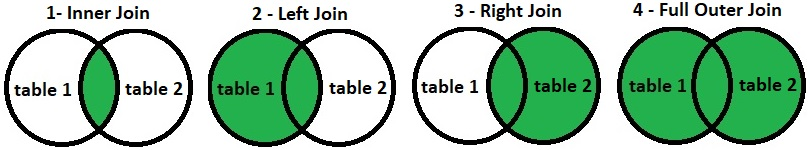
\includegraphics[width=15cm]{types-of-joins}}}
\end{figure}
\begin{lstlisting}[language=SQL]
-- Contents: Comma, (Inner) Join, Left (Outer) Join, Right (Outer) Join,, FUll (Outer) Join, Cross Join

-- Comma
select	*
from	author a, book b
where	a.author_id = b.author_id
; -- 67 results - but we have 69 books? (because 2 books have null author_id)

-- (Inner) Join
select	*
from	author a
join	book b -- or replace with equivalent: inner join
on		a.author_id = b.author_id
; -- again 67 same results
-- Join will shows all results that exist both in left (author) and right (book) table
-- In simple words in this case it produces a table with all authors who have at least one book and their books

-- Left (Outer) Join
select		*
from		author a
left join	book b -- or replace with equivalent: left outer join
on			a.author_id = b.author_id
; -- now 68 results
-- Why? Left Join shows all results of the left (author) table, even if there is no match in right (book) table
-- Notice Virginia Woolf appears in results and book columns are populated with null, since she has no book associated with her
-- In simple words in this case it produces a table with all authors even if they don't have any book and their books

-- Right (Outer) Join
select		*
from		author a
right join	book b -- or replace with equivalent: right outer join
on			a.author_id = b.author_id
; -- now 69 results
-- Why? Right Join shows all results of the right (book) table, even if there is no match in left (author) table
-- Notice books 'The SQL Cook Book' and 'Novel Nook Murders' have no author details, because we didn't associate them with any author

-- Full Join - MySQL doesn't support Full Join
-- How can it be achieved?
select		*
from		author a1
left join	book b1
on			a1.author_id = b1.author_id
union
select		*
from		author a2
right join	book b2
on			a2.author_id = b2.author_id
; -- now 70 results
-- Why? Full Join shows all results of the left (author) and the right (book) table, even if there is no match in the other table
-- Notice now books 'The SQL Cook Book' and 'Novel Nook Murders' and author Virginia Woolf show in results even though they have no much
-- Note: Union combines the results returned by two queries, we will see it better later

-- Cross Join (Cartesian Join)
select		*
from		author a
cross join	book b
; -- 1449 results
-- Why? Cross Join will match every row from table left table, with every row from table right table
-- This kind of join is rarely used

-- Note: Difference between Join and Cross Join is that on Join we should use on to define how rows will be matched from one table with the other ones while Cross Join there should be no on conditions
-- Some DBMS like MySQL allow (Inner) Join without on condition and Cross Join with on
\end{lstlisting}
\subsection{Union/Union All/Intersect/Minus}
\begin{itemize}
	\item \textbf{Union:} returns the joined result set of two or more selects, distinct values only.
	\item \textbf{Union All:} returns the joined result set of two or more selects, allows duplicates.
	\item \textbf{Intersect:} returns the common distinct rows of two or more selects.
	\item \textbf{Minus:} returns the result set that exists on first select, but not on the second select .
\end{itemize}
\begin{lstlisting}[language=SQL]
-- Contents: Union/Union Al/Intersect/Minus

-- Union/Union All
-- Union operator is used to join the result set of two or more select statements
-- The data all selects under union return must have same structure (number of columns, order and similar data types)
-- Union vs Union All: Union selects distinct values while union all allows duplicates
create table tmp_numbers_a (num_x int, num_y int);
create table tmp_numbers_b (num_k int, num_l int);
insert into tmp_numbers_a values (1, 2), (2, 3), (3, 4), (4, 5), (1, 2);
insert into tmp_numbers_b values (1, 2), (2, 3), (3, 5), (5, 8);
commit;

-- Union
select * from tmp_numbers_a
union
select * from tmp_numbers_b; -- 6 rows, notice no duplicate values inserted in the result set

-- Union All
select * from tmp_numbers_a
union all
select * from tmp_numbers_b; -- 9 rows, notice all results from both tables are inserted now, even duplicates

-- Intersect
select * from tmp_numbers_a
intersect
select * from tmp_numbers_b; -- 9 rows, notice all results from both tables are inserted now, even duplicates
-- Intersect returns the distinct common values between two or more tables
-- Similarly to union, the column number, order and datatype has to be the same

-- alternatively without intersect keyword
select	distinct num_x, num_y
from	tmp_numbers_a
where	(num_x, num_y) in (
select * from tmp_numbers_b)
;

drop table tmp_numbers_a;
drop table tmp_numbers_b;

-- Minus - is Oracle Based, this won't work in MySQL
select author_id from author
minus
select author_id from book;
-- This will select all author ids from table author, except the ones that exist in table book
-- In simple words, it will find all author ids that don't have a book
-- How can we achieve the same without minus?
select a.author_id from	author a
where a.author_id not in (
select distinct b.author_id from book b where b.author_id is not null
);
-- Notice the is not null for b.author_id.alter
-- This is important because if you place null value inside () for in or not in, then it will never show any results
\end{lstlisting}
\subsection{Joins vs Union/Intersect/Minus Operators}
\paragraph{} With joins the final result set, consists of rows that have the columns from all the joined tables. While with Union and the other operators, the columns of the selects has to be the same and the final result will contain the same columns, but different result set (rows). They are not the same, it's important to understand this difference now from the previous examples.
\subsection{Subquery}
\begin{lstlisting}[language=SQL]
-- Example:
select	a.author_id from	author a
where	a.author_id not in (
			select distinct b.author_id from book b where b.author_id is not null
);
\end{lstlisting}
\subsection{Types of SQL Functions}
\paragraph{} Functions are code snippets that can be used to perform various operations on the data. These functions don't change the data, only how we view them. There are three types of SQL Functions:
\begin{itemize}
	\item \textbf{Aggregate Functions:} operate on groups of rows and produce a single result/row for each group.
	\item \textbf{Non Aggregate Functions:} operate on each row separately and produce one result for each row.
	\item \textbf{Analytic Functions:} operate on groups of rows and produce one result for each group of rows, but in contrast to aggregate functions they return multiple results/rows for each group.
\end{itemize}
\subsection{Aggregate Functions}
\begin{lstlisting}[language=SQL]
-- Content: group by/count/having/max/min/limit/avg/sum

-- group by: groups the selected results based on column(s)
-- count: counts how many results are found

-- Note:
-- 1. count(*) -> will also include in count null values
-- 2. count(column) -> will count how many non null values are found for that column
-- 3. count(distinct column) -> will only count how many non null distinct values that column has

-- let's find all how many books each author has (even if one author has no books)
select		a.first_name, a.last_name, count(b.book_id) number_of_books -- print only first, last name and number of books
from		author a
left join	book b
on			a.author_id = b.author_id -- Up to here we just joined the all authors with their books
group by	a.author_id -- now we group by the results by author_id
order by	number_of_books desc -- optional just to order the results based on the number of books
;
-- Note: We can select specific columns only from table author because in group by we used the primary key author_id from that table
-- otherwise we can only use the columns included in group by clause and the results of aggregate functions

-- Having: like where clause but only for group by/aggregated conditions

-- Find all authors that have more than 5 books (not 5)
select		a.first_name, a.last_name, count(b.book_id) number_of_books -- print only first, last name and number of books
from		author a
left join	book b
on			a.author_id = b.author_id -- Up to here we just joined the all authors with their books
group by	a.author_id -- now we group by the results by author_id
having		number_of_books > 5
order by	number_of_books desc -- optional just to order the results based on the number of books
;

-- max/min: maximum/minimum value of a column

-- Find the youngest author
select max(birthday) from author;
-- Find the oldest author
select min(birthday) from author;

-- limit #: limit the number of results (MySQL only, other DBMS have their own way of achieving this)

-- Find the author with most books
select		a.first_name, a.last_name, count(b.book_id) number_of_books -- print only first, last name and number of books
from		author a
left join	book b
on			a.author_id = b.author_id -- Up to here we just joined the all authors with their books
group by	a.author_id -- now we group by the results by author_id
order by	number_of_books desc
limit		1; -- MySQL only

select * from author;
select * from author limit 1, 4; -- will fetch 4 rows, starting from row num: 1. Note: first row num is 0.
select * from author limit 3; -- is equal to
select * from author limit 0, 3;

-- avg: calculates the average value of the column

-- Find the average number of books per author
select avg(number_of_books)
from (
select		a.first_name, a.last_name, count(b.book_id) number_of_books -- print only first, last name and number of books
from		author a
left join	book b
on			a.author_id = b.author_id -- Up to here we just joined the all authors with their books
group by	a.author_id -- now we group by the results by author_id
) authors_book_count;

-- sum: calculates the sum of the values of the column

-- Find the total number of books
select sum(number_of_books)
from (
select		a.first_name, a.last_name, count(b.book_id) number_of_books -- print only first, last name and number of books
from		author a
left join	book b
on			a.author_id = b.author_id -- Up to here we just joined the all authors with their books
group by	a.author_id -- now we group by the results by author_id
) authors_book_count;

-- Note: In above results there is one small issue: the books without author are not included
-- if we wanted that we would have to use the long syntax of full join
\end{lstlisting}
\subsection{Non-Aggregate Functions - String Functions}
\begin{lstlisting}[language=SQL]
-- Content: concat/upper/lower/reverse/replace/substring

-- concat: concatenates two or more strings
select first_name, last_name, concat(first_name, ' ', last_name) as full_name from author;

-- upper/lower: changes letters to uppercase/lowercase
-- reverse: reverses the order of the letters
select upper(first_name), lower(last_name), reverse(concat(first_name, ' ', last_name)) as full_name from author;
-- notice you can pass the result of one function to another one

-- replace: replace pattern from string with another string
select replace(title, ' ', '-') as full_name from book; -- replace spaces with - in book titles

-- substring(text, start, length); note: if start is negative number, it starts from the end and moves towards the right
select title, substring(title, 1, 3) substr_title from book;
select title, substring(title, -2, 3) substr_title from book; -- only two characters exist since we did -2, so no 3d to show
select title, substring(title, -3, 3) substr_title from book;
select title, substring(title, -5, 5) substr_title from book; -- notice what happens to titles that have less characters than star position
\end{lstlisting}
\subsection{Non-Aggregate Functions - Date Functions}
\begin{lstlisting}[language=SQL]
-- Content: now/sysdate/curdate/curtime/interval

-- now() vs sysdate()
-- sysdate/now: sysdate returns the date-time it executes while now returns a constant time, at which the statement began to execute

-- curdate/curtime: curdate returns only the current date while curtime only the current timestamp

select now(), sysdate(), curdate(), curtime();

-- Example: sysdate vs now
select	sysdate(), sleep(5), sysdate(),
now(), sleep(5), now()
; -- notice: sysdate returns different values in each call while now the same timestamp

-- Why it matters? Imagine you want to update more than one columns with current datetime but the query takes time to complete, there will be small difference in timestamp between the two dates, so in such cases now is more suitable

-- To Compare Dates you use normally comparison operators: >, >=, <, <=, =

-- Find the books that where released after the death of their author
select	*
from	author a
join	book b
on		a.author_id = b.author_id
where	deathday is not null
and year(deathday) < release_year
; -- year is MySQL specific. Note: with year we extract the year part of the date since release_year is just the year we can't directly compare these without year

-- If one database doesn't support year function, you can use substring to extract only the part you need

-- interval
select sysdate(), sysdate() + interval 2 day;
select sysdate(), sysdate() + interval 1 month;
select sysdate(), sysdate() - interval 1 year;
select sysdate(), sysdate() + interval 1 hour;
\end{lstlisting}
\subsection{Coalesce/ifnull/NVL/isnull/Case Expression and Cast}
\begin{lstlisting}[language=SQL]
-- Content: coalesce/ifnull/nvl/isnull/case/cast

-- coalesce, ifnull, nvl: all will return the first (from left) non null values
-- difference: ifnull and nvl can take only two parameters, while coalesce can take more than two

-- if deathday is not null, it will take that value, else it will take the next one, birthday
select deathday, birthday, ifnull(deathday, birthday) deathday_else_birthday from author;
select deathday, birthday, nvl(deathday, birthday) deathday_else_birthday from author; -- nvl is Oracle based
select deathday, birthday, coalesce(deathday, birthday) deathday_else_birthday from author;

-- isnull: returns 1 if given value is null else 0
select isnull(null);

-- Case Expression
-- Syntax: case when condition1 then result1 when condition2 then result2 .... else result end
select deathday, birthday, case when deathday is null then birthday else deathday end deathday_else_birthday from author;

-- another example
select		a.first_name, a.last_name, count(b.book_id) number_of_books, -- print only first, last name and number of books
(case
when count(b.book_id) = 0 then ''
when count(b.book_id) < 3 then '*'
when count(b.book_id) < 6 then '**'
when count(b.book_id) < 9 then '***'
else '****'
end) as stars
from		author a
left join	book b
on			a.author_id = b.author_id -- Up to here we just joined the all authors with their books
group by	a.author_id -- now we group by the results by author_id
order by	number_of_books desc -- optional just to order the results based on the number of books
;

-- cast is used to convert the data from one data type to another
select cast(14 as char);
select cast('2023-03-14' as date);
\end{lstlisting}
\subsection{Section Notes}
\begin{itemize}
	\item For all \acs{SQL}/\acs{DQL} commands of this section \href{file:./source-items/sql/4-sql-dql.sql}{click here}.
	\item For more on MySQL Datatypes \href{https://dev.mysql.com/doc/refman/8.0/en/data-types.html}{click here}.
	\item For more on \acs{SQL} Functions \href{https://dev.mysql.com/doc/refman/8.0/en/functions.html}{click here}.
\end{itemize}


\section{Transactions Theory}
\subsection{Transaction Definition}
\paragraph{} A \textbf{Transaction} is a set of multiple operations performed on the database as a single logical unit; taking place as a whole or not at all. Transactions allow correct recovery from failures and keep the database consistent even in case of system failure.
\subsection{\acs{ACID} Properties}
\paragraph{\acf{ACID}} These four database transaction properties ensure the correctness of a transaction even during system failures.
\begin{itemize}
	\item \textbf{Atomicity} says that all SQL operations within a transaction are treated as a single logical unit of work, which can either succeed or fail as a whole.
	\item \textbf{Consistency} ensures that one transaction will only bring the database from one consistent state to another, preserving database invariants. Any changes made to the database must be valid according to all defined rules: constraints, cascades, triggers and their combination. Referential integrity guarantees the primary-foreign key relationship.
	\item \textbf{Isolation}; Transactions happen concurrently (multiple transactions read and write to a table at the same time). Isolation ensures that concurrent execution of transactions leaves the database in the same state that would have been if the transactions were executed sequentially. Isolation is the main goal of concurrency control; depending on the isolation level used, the effects of an incomplete transaction may or may not be visible to other transactions.
	\item \textbf{Durability} is the property which ensures that the changes of a successful transaction, once committed; are permanent and should remain even in case of system failure.
\end{itemize}
\paragraph{} For more on \acs{ACID} please see here: \href{https://en.wikipedia.org/wiki/ACID}{\acs{ACID} - Wikipedia} and here: \href{https://dev.mysql.com/doc/refman/8.0/en/mysql-acid.html}{MySQL - ACID}.
\paragraph{} For more on Concurrency Control please see here: \href{https://en.wikipedia.org/wiki/Concurrency_control}{Concurrency Control - Wikipedia}.
\subsection{Transaction Isolation Read Phenomena}
\paragraph{} \textbf{Read phenomena} refers to three different read phenomena, when one transaction retrieves data that another transaction may have updated.
\begin{itemize}
	\item \textbf{Dirty Reads}. A Dirty Read (uncommitted dependency) occurs when one transaction retrieves data that have been changed by another transaction that are not yet committed.
	\item \textbf{Non-Repeatable Reads}.  A Non Repeatable Read occurs when a transaction retrieves a set of data more than once, but reads different data each time because other transactions have changed them.
	\item \textbf{Phantom Reads}. A Phantom Read occurs when a transaction retrieves a set of data more than once, sees same data each time, however other transactions have changed them.
\end{itemize}
\subsection{Transaction Isolation Levels}
\paragraph{} The aim of \textbf{Transaction Isolation Levels} is to control the behavior of concurrent transactions. There are four isolation levels:
\begin{itemize}
	\item \textbf{Read Uncommitted} or \textbf{Dirty Reads}. The lowest isolation level. In this level, one transaction may see not yet committed changes made by other transactions.\\\textbf{Concurrency Effects:} Dirty Reads, Non-Repeatable Reads and Phantom Reads.\\\textbf{Solves:} -.
	\item \textbf{Read Committed}. In this isolation level, the transaction will see only committed changes by other transactions.\\\textbf{Concurrency Effects:} Non-Repeatable Reads and Phantom Reads.\\\textbf{Solves:} Dirty Reads.
	\item \textbf{Repeatable Reads}. Guarantees that already retrieved data will be the same in that transaction if retrieved again, even if they are changed by other transactions.\\\textbf{Concurrency Effects:} Phantom Reads.\\\textbf{Solves:} Dirty Reads, Non-Repeatable Reads.
	\item \textbf{Serializable} is the highest isolation level. This isolation level blocks other transactions from changing retrieved data.\\\textbf{Concurrency Effects:} Higher chances for deadlocks.\\\textbf{Solves:} Dirty Reads, Non-Repeatable Reads, Phantom Reads.
\end{itemize}
\paragraph{} A lower isolation level increases concurrency and performance but can result in data inconsistencies. On the other hand, higher isolation increases data consistency but also decreases concurrency and performance. Also Deadlocks may occur more often the higher the isolation level is.
\paragraph{} The default isolation level varies on each \acs{DBMS}.
\subsection{Starvation and Deadlock}
\paragraph{} \textbf{Starvation} is a problem in concurrent computing where a process is continuously denied access to necessary resources to complete its task.
\paragraph{} \textbf{Deadlock} is a form of \textbf{Starvation}. Deadlock can occur for example when Transaction 1 requires to lock resources A and B, acquires lock for Resource A but resource B is already locked by another Transaction 2 and the Transaction 2 also requires to lock Resource A which is already locked by Transaction 1. As a result neither transaction can complete until the other one releases the acquired resource.
\paragraph{} Some \acs{DBMS} don't use locks for concurrency control but \textbf{Snapshots}. For more on this please see: \href{https://en.wikipedia.org/wiki/Snapshot_isolation}{Snapshot Isolation - Wikipedia}.
\paragraph{} For more on Isolation Levels please see here: \href{https://en.wikipedia.org/wiki/Isolation_(database_systems)}{Isolation Levels - Wikipedia}.
\subsection{Types of Locks (Lock Modes) \& Levels of Locking in \acs{DBMS}}
\paragraph{} \textbf{Database Hierarchy}\\Database $\rightarrow$ Table space $\rightarrow$ Table $\rightarrow$ Partition $\rightarrow$ Page $\rightarrow$ Tuple (Row/Record)
\paragraph{} \textbf{There are four levels of locking in \acs{DBMS}}
\begin{itemize}
	\item \textbf{Database Level}: Full database is locked. Not suitable for multi-user \acs{DBMS}.
	\item \textbf{Table Level}: Full table is locked. Not suitable for multi-user \acs{DBMS}.
	\item \textbf{Page Level}: The page always consists of a fixed size. A table can span to several pages and each page can contain several records/rows. Suitable for multi-user \acs{DBMS}.
	\item \textbf{Row Level}: Locks only single rows. It is less restrictive but more resource costly.
\end{itemize}
\paragraph{} \textbf{Types of Locks (Lock Modes)}
\subparagraph{} \textbf{Page and Row Lock Modes}
\begin{itemize}
	\item \textbf{X lock (Exclusive):} This lock type ensures that a page or row will be reserved exclusively for the transaction that imposed the exclusive lock, as long as the transaction holds the lock.\\The Exclusive lock will be imposed by the transaction when it wants to modify the page or row data, which is in the case of DML statements INSERT, DELETE, UPDATE.\\An exclusive lock can only be imposed to a page or row, only if there is no other exclusive or shared lock for that page or row.
	\item \textbf{S lock (Shared):} This lock will reserve a page or row only for reading, which means any other transaction will be prevented from modifying the locked page or row as long as the lock is active. A shared lock can be imposed many times at the same page or record at the same time.
	\item \textbf{U lock (Update):} Is similar to exclusive lock but is designed to be more flexible. It can be imposed only on a page or row that already has a shared lock. Once the transaction that holds the update lock is ready to change the data, the lock will be changed to an exclusive lock.
	\item \textbf{Note:} X, S and U locks can also be used on higher level \acs{DB} objects like table or tablespace, but it is not recommended.
\end{itemize}
\subparagraph{} \textbf{Table Space, Table and Partition Lock Modes}
\begin{itemize}
	\item \textbf{I lock (Intent):} This kind of lock is a means used by a transaction to inform other transactions about its intention to acquire a lock. When a transaction wants to acquire a lock on a row, it will first acquire an intention lock on the table. This is very important from performance aspect, as the \acs{DBMS} will only inspect Intent Locks on table level to check if it's possible to acquire the lock, without having to check each page/row.
	\item \textbf{IX lock (Intent Exclusive):} Indicates that the transaction has the intention to modify lower hierarchy resources by acquiring X locks individually on them.
	\item \textbf{IS lock (Intent Shared):} Similar to IX, but for intention to read only.
	\item \textbf{IU lock (Intent Update):} Can be acquired only at page level and as soon as the operation takes place it is converted to IX lock.
\end{itemize}
\paragraph{}
\begin{itemize}
	\item For more on locks please see here: \href{https://dev.mysql.com/doc/refman/8.0/en/innodb-locking.html}{InnoDB Locking - MySQL}.
	\item For more on table locks see here: \href{https://dev.mysql.com/doc/refman/8.0/en/lock-tables.html}{Table Locks - MySQL}.
\end{itemize}


\section{\acs{TCL} Commands In Depth}
\paragraph{} In this section we will cover the \acf{TCL} commands. These commands deal with the behavior of transactions.\\\textbf{Purpose:} Define the behavior of transactions.\\\textbf{Auto-Commit:} -.
\subsection{Commit/Rollback}
\begin{lstlisting}[language=SQL]
	commit; -- data changes made via DML commands in current session will be made permanent
	rollback; -- non committed data changes made via DML commands in current session will be reverted
	
	-- Note: commit/rollback have no impact on what is done in other sessions
\end{lstlisting}
\subsection{Implicit Commit}
\paragraph{} In previous section we saw the commit and rollback commands, which explicitly save or revert changes done by \acs{DML} commands. However, there are other \acs{SQL} commands, that if run, they will implicitly end any pending transaction in session and silently commit unsaved changes.
\begin{itemize}
	\item \acs{DDL} commands
	\item Some \acs{TCL} commands (Start Transaction/Begin Work/Begin)
	\item General Rule: Any command that auto-commits.
\end{itemize}
\paragraph{} So it's advised, if there are uncommitted changes, before running \acs{SQL} commands other than \acs{DML} and \acs{DQL}, either (1) commit/rollback or (2) open a new session and execute these commands there to avoid accidentally committing unwanted changes.
\begin{lstlisting}[language=SQL]
	-- Example of Implicit Commit
	
	select * from book where title = 'Experimental Cooking Recipes'; -- no such book initially
	
	start transaction;
	insert into book (title, release_year, book_language) values ('Experimental Cooking Recipes', 2004, 'English');
	-- if you check before rollback book will be there, run rollback and check again, book won't be there anymore
	rollback;
	
	-- now we will try again the same as above, but before rollback we will run DQL command create table
	
	start transaction;
	insert into book (title, release_year, book_language) values ('Experimental Cooking Recipes', 2004, 'English');
	create table tmp (tmp_id int primary key, value varchar(10)); -- now before rollback run this DQL command
	rollback;
	
	-- now book remains even after rollback - this is because DQL commands like create/drop table autocommit
	
	drop table tmp; -- we no longed need this table
\end{lstlisting}
\subsection{Start Transaction/Begin Work/Begin}
\paragraph{} One thing to note is that in some \acs{DBMS} start transaction is silently executed each time any \acs{DML} command is executed (like in Oracle SQL) but in other ones like MySQL this does not happen (by default) unless you explicitly start a transaction, else any \acs{DML} command is considered as a single transaction that will be auto-committed once executed. Solutions in systems like MySQL:
\begin{itemize}
	\item Explicitly start a transaction each time
	\item Disable auto-commit session variable (set autocommit = 0;)
	\item Disable auto-commit global variable (set global autocommit = 0;) and start a new session
	\subitem Note: In MySQL Workbench you also have to change the below setting:
	\subitem Edit -> Preferences -> SQL Execution -> Uncheck option: New connections use auto commit mode
	\subitem Otherwise global variable autocommit is ignored
\end{itemize}
\paragraph{} We will work by explicitly starting a new transaction each time.
\begin{lstlisting}[language=SQL]
	-- start transaction = begin work = begin. They do the same thing, start a new transaction
	-- running these commands will disable auto-commit setting for DML commands if it's enabled, until transaction is completed (by commit/rollback or implicit commit)
	
	start transaction;
	-- execute DQL/DML commands
	commit; -- or rollback;
	
	-- or
	begin work;
	-- execute DQL/DML commands
	commit; -- or rollback;
	
	-- or
	begin;
	-- execute DQL/DML commands
	commit; -- or rollback;
\end{lstlisting}
\subsection{Rollback to Savepoint}
\begin{lstlisting}[language=SQL]
	-- Syntax:
	start transaction;
	-- execute DQL/DML commands
	savepoint pointA; -- pointA can be any valid name you wish
	-- execute DQL/DML commands
	savepoint pointB;
	-- execute DQL/DML commands
	-- ..
	rollback to savepointA; -- or to any other savepoint you wish to revert to
	-- this will result in changes done up to save pointA to be committed
	-- but any changes after pointA are reverted
	commit;
	
	-- Example:
	start transaction;
	
	select * from book where title = 'Experimental Cooking Recipes'; -- we have this book from before
	-- change publisher
	update book set release_year = 2014 where title = 'Experimental Cooking Recipes';
	select * from book where title = 'Experimental Cooking Recipes'; -- see updated release year
	savepoint pointUpdate;
	
	delete from book where title = 'Experimental Cooking Recipes'; -- book is deleted
	select * from book where title = 'Experimental Cooking Recipes'; -- no such book
	savepoint pointDelete;
	
	rollback to pointUpdate; -- keep changes up to that save point and revert anything done below that point
	commit;
	
	select * from book where title = 'Experimental Cooking Recipes'; -- book will be there with updated release year
\end{lstlisting}
\subsection{Access Modes: Read Write/Read Only}
\paragraph{} There are two transaction access modes: 1. READ WRITE (default) and READ ONLY. READ WRITE access mode allows you to execute both \acs{DQL} and \acs{DML} commands within a transaction while READ ONLY allows you to execute only \acs{DQL} queries. By default a transaction is in READ WRITE access mode.
\begin{lstlisting}[language=SQL]
	-- Syntax:
	start transaction read only;
	
	start transaction read write;
	start transaction; -- by default this will also get read write access mode
	
	-- Example
	start transaction read only;
	select * from book where title = 'Experimental Cooking Recipes'; -- book will be there with updated release year
	update book set release_year = 2013 where title = 'Experimental Cooking Recipes'; -- this or any other DML command (insert/update/delete) will fail
	commit;
	
	start transaction read write; -- or start transaction; has the same access mode
	select * from book where title = 'Experimental Cooking Recipes'; -- book will be there with updated release year
	update book set release_year = 2013 where title = 'Experimental Cooking Recipes'; -- now both commands will work
	commit;
\end{lstlisting}
\subsection{Intro to Transaction Isolation Levels}
\paragraph{} In below sections we will see in action the transaction isolation levels we saw in the previous section. To understand the effect of isolation levels we will be working on more than one session in below sections.\\\textbf{Note:} Transaction Isolation Level can only be set before transaction starts, not during.
\subsection{Practice: Transaction Isolation Levels - Read Uncommitted}
\begin{lstlisting}[language=SQL]
	-- Read uncommitted else dirty reads: this isolation level allows you to see changes that are not yet committed
	-- Lowest Isolation Level
	-- Effects: (1) Dirty Reads, (2) Non Repetable Reads (3) Phantom Reads
	-- Solves: -
	
	-- Session A: Start
	start transaction;
	select * from book where title = 'Experimental Cooking Recipes';
	-- change release year from 2013 to 2015
	update book set release_year = 2015 where title = 'Experimental Cooking Recipes';
	-- before commit - go to part Session B
	commit; -- once steps on Session B are done, do commit
	-- Session A: End
	
	-- Copy the content of Session B in another session
	-- Session B: Start
	set transaction isolation level read uncommitted;
	start transaction; -- now isolation level is set to read uncommitted
	-- release year will be 2015, even though change is not committed yet
	select * from book where title = 'Experimental Cooking Recipes';
	commit;
	-- Session B: End
\end{lstlisting}
\subsection{Practice: Transaction Isolation Levels - Read Committed}
\begin{lstlisting}[language=SQL]
	-- Read committed: this isolation level allows you to only see committed changes
	-- Second Lowest Isolation Level
	-- Effects: (1) Non Repeatable Reads (2) Phantom Reads
	-- Solves: (1) Dirty Reads (Uncommitted Changes)
	
	-- Non Repeatable Reads: Same query in one transaction will read different values due to changes made by a different transaction
	
	-- Session A.1: Start
	-- go to Session B.1
	-- Session A.1: End
	
	-- Session A.2: Start
	start transaction;
	update book set release_year = 2005 where title = 'Experimental Cooking Recipes';
	commit;
	-- go to Session B.2
	-- Session A.2: End
	
	-- Session A.3: Start
	start transaction;
	update book set release_year = 2035 where title = 'Experimental Cooking Recipes';
	commit;
	-- go to Session B.3
	-- Session A.3: End
	
	-- Copy the content of Session B in another session
	-- Session B: Start
	
	-- Session B.1: Start
	set transaction isolation level read committed; -- set transaction isolation level to read committed
	start transaction;
	select * from book where title = 'Experimental Cooking Recipes'; -- release year is 2015
	-- go to section A.2
	-- Session B.1: End
	
	-- Session B.2: Start
	select * from book where title = 'Experimental Cooking Recipes'; -- release year is 2005
	-- go to section A.3
	-- Session B.2: End
	
	-- Session B.3: Start
	select * from book where title = 'Experimental Cooking Recipes'; -- release year is 2035
	commit;
	-- Session B.3: End
	
	-- Notice that at each select in same transaction we read different value for release year.
	
	-- Session B: End
\end{lstlisting}
\subsection{Practice: Transaction Isolation Levels - Repeatable Read}
\begin{lstlisting}[language=SQL]
	-- Repeatable read: Guarantees that in one transaction, same query will return same
	-- values, even if they are updated by another transaction 
	-- Effects: (1) Phantom Reads
	-- Solves: (1) Dirty Reads (Uncommitted Changes) (2) Non Repeatable Reads
	
	-- Session A.1: Start
	-- go to Session B.1
	-- Session A.1: End
	
	-- Session A.2: Start
	start transaction;
	update book set release_year = 2008 where title = 'Experimental Cooking Recipes';
	commit;
	-- go to Session B.2
	-- Session A.2: End
	
	-- Copy the content of Session B in another session
	-- Session B: Start
	
	-- Session B.1: Start
	set transaction isolation level repeatable read; -- set transaction isolation level to repeatable read
	start transaction;
	select * from book where title = 'Experimental Cooking Recipes'; -- release year is 2035
	-- go to section A.2
	-- Session B.1: End
	
	-- Session B.2: Start
	select * from book where title = 'Experimental Cooking Recipes'; -- release year is still 2035
	commit;
	start transaction;
	select * from book where title = 'Experimental Cooking Recipes'; -- now new transaction sees updated value (release year 2008)
	commit;
	-- Session B.2: End
	
	-- Even though value is updated and committed at another transaction,
	-- this isolation level guarantees that results will be the same
	
	-- Session B: End
\end{lstlisting}
\subsection{Practice: Transaction Isolation Levels - Serializable}
\begin{lstlisting}[language=SQL]
	-- Serialable: Prevents other transactions from updating data this transaction has acquired lock on
	-- Highest Isolation Level
	-- Effects: -
	-- Solves: (1) Dirty Reads (Uncommitted Changes) (2) Non Repeatable Reads (3) Phantom Reads
	
	-- Phantom Reads: One transaction works on a set of data, that transaction keeps seeing exactly same data
	-- during its execution, however other transactions are allowed to change them (insert/delete/update). 
	-- Serializable prevents this.
	
	-- Note: If a transaction on Isolation Level: REPEATABLE READ makes change on some data (for example delete) then another transaction on Isolation Level: Serializable reads these data and then the previous transaction commits the change, the latest transaction still sees inconsistent data.
	
	-- Session A.1: Start
	-- go to Session B.1
	-- Session A.1: End
	
	-- Session A.2: Start
	start transaction;
	select * from book where release_year > 1980 and release_year < 1990; -- works
	update book set release_year = 18 where release_year = 1980; -- fails because table is locked
	delete from book where release_year = 1980; -- fails because table is locked
	insert into book (title, release_year, book_language) values ('New SQL Book', 2004, 'English'); -- fails again
	-- below works because only table book was used and thus locked by the other transaction
	select * from author where first_name in ('Virginia', 'John');
	insert into author (first_name, last_name, birthday) values ('John', 'Wick', '1891-04-14');
	update author set birthday = '1883-01-25' where first_name = 'Virginia' and last_name = 'Wolf';
	update author set birthday = '1882-01-25' where first_name = 'Virginia' and last_name = 'Wolf';
	delete from author where first_name in ('Virginia', 'John');
	commit;
	-- go to B.2
	-- Session A.2: End
	
	-- Copy the content of Session B in another session
	-- Session B: Start
	
	-- Session B.1: Start
	set transaction isolation level serializable; -- set transaction isolation level to serializable
	start transaction;
	select * from book where release_year > 1980 and release_year < 1990; -- works
	-- go to section A.2
	-- Session B.1: End
	
	-- Session B.2: Start
	commit;
	-- go again to A.2, now they will work again
	-- Session B.2: End
	
	-- Session B: End
	
	-- Note: The precise way of locking varies based on DBMS and its configuration.
\end{lstlisting}
\subsection{Transaction Management}
\begin{lstlisting}[language=SQL]
	-- View transactions
	-- MySQL Syntax:
	select	*
	from	performance_schema.events_transactions_current
	where	state not in ('COMMITTED', 'ROLLED BACK');
\end{lstlisting}
\subsection{Section Notes}
\begin{itemize}
	\item For all \acs{SQL}/\acs{TCL} commands of this section \href{file:./source-items/sql/5-sql-tcl.sql}{click here}.
	\item For more on \acs{SQL} \acs{TCL} \href{https://dev.mysql.com/doc/refman/8.0/en/sql-transactional-statements.html}{click here}.
\end{itemize}


\section{Extras}
\subsection{Database Object Hierarchy}
\begin{enumerate}
	\item \textbf{\acs{DBMS}:} The software that contains the databases and provides the ways we can interact with it.
	\item \textbf{\acl{DB}:} Contains all the objects of the database (Tables/Triggers/Sequences/etc).
	\item \textbf{Tablespace}: Contains tables, indexes and other large objects and data. It is used to organize the \acs{DB} into logical groups.
	\item \textbf{Table}: Is used to store data that have a specific structure.
	\item \textbf{Partition}: A table is split into partitions (when it contains a lot of data).
\end{enumerate}
\subsection{SQL Hints}
\subsection{DB Links}
\paragraph{} Note that currently DB Links are not supported by MySQL. We will only see a few basic things about how they work in Oracle \acs{SQL}.
\begin{lstlisting}[language=SQL]
-- DB Links allow a DB user to access another database

select * from dba_db_links; -- all DB links defined in the database
select * from all_db_links; -- all DB links that current user has access to
select * from user_db_links; -- all DB links owned by current user

-- Private vs Public DB Links
-- Private DB Links can be used only by their owner
-- Public DB Links can be used by any DB user assuming the user has privileges to access the other database

-- Create Public DB Link
create public database link dblink
connect to product_db_username identified by product_db_password
using '<oracle_sid>'; -- sid: service id

-- Create Private DB Link
create database link dblink
connect to product_db_username identified by product_db_password
using '<oracle_sid>'; -- sid: service id

-- Using DB Links
select * from tablename@dblink; -- tablename any table from remote db and @ means what follows is a db link
\end{lstlisting}
\subsection{Performance Tips}
\paragraph{} When working in real production databases with millions of records, it is important to understand the performance of the queries you write and optimize them as much as possible. In this section we will see some tips about this.
\begin{itemize}
	\item Use Partition and Primary Keys.
	\item Limit fetched results from tables using conditions in where clause.
	\item Select only required columns from tables.
	\item Use same datatype in conditions in where clause.
	\item Use SQL Hints.
	\item Use Explain.
\end{itemize}
\paragraph{} Now let's understand the above in detail:
\begin{itemize}
	\item \textbf{Use Partition and Primary Keys.} This is the most important part to speed up query execution. Tables are split into partitions. By using Partition and Primary Keys, the \acs{DBMS} will know in which partition to search into and thus limiting a lot the data it will search to.
	\item \textbf{Limit fetched results from tables using conditions in where clause.} This is important, especially when joining many tables together, to limit the results fetched from each table as much as possible.
	\item \textbf{Select only required columns from tables.} In real databases, tables can consist of many columns, and some columns may hold large data. Loading every column can impact performance and use more resources on the system. Especially columns with large data should be avoided as much as possible.
	\item \textbf{Use same datatype in conditions in where clause.} For example, if one column has stored numbers as varchar(5) in your query you should do select * from table where columnA = \lq12345\rq; and not select * from table where columnA = 12345;. While both work, if you run the second query, it will cause the DBMS to convert each fetched row from char to number. In a huge database this can be a significant slowdown factor.
	\item \textbf{Use SQL Hints} to instruct the \acs{DB} engine how to execute the query. The \acs{DB} engine does optimize the queries, but not always in the best possible way.
	\item \textbf{Use Explain} to understand the complexity of the query before running it.
	\begin{lstlisting}[language=SQL]
-- Use explain to see the complexity of below query
select		a.first_name, a.last_name, count(b.book_id) number_of_books -- print only first, last name and number of books
from		author a
left join	book b
on			a.author_id = b.author_id -- Up to here we just joined the all authors with their books
group by	a.author_id -- now we group by the results by author_id
order by	number_of_books desc
limit		1; -- MySQL only

-- Explain
explain
select		a.first_name, a.last_name, count(b.book_id) number_of_books -- print only first, last name and number of books
from		author a
left join	book b
on			a.author_id = b.author_id -- Up to here we just joined the all authors with their books
group by	a.author_id -- now we group by the results by author_id
order by	number_of_books desc
limit		1; -- MySQL only
	\end{lstlisting}
\end{itemize}
\subsection{Global and Session Variables}
\paragraph{} On SQL there are two scopes for System Variables: 1. Session and 2. Global. The session variables affect the operation of the individual client connection only, while global variables will affect all new client sessions that will start after the change takes effect. When the server starts, it loads the default values to global variables and then session variables are initialized from the global variables.
\begin{lstlisting}[language=SQL]
-- Global Variables
select @@global.autocommit; -- check default initial value

set global autocommit = 0; -- change to 0 or 1 based on what you had before and see it changed to the new value
set @@global.autocommit = 0;
-- Try to restart the session or even the server and see the global variable is the same
set @@global.autocommit = 1; -- revert to orinal value again - for me it was 151

-- Persisting Global Variables to mysqld-auto.cnf - these values will be loaded to global variables upon server restart
set persist autocommit = 0;
set @@persist.autocommit = 0;

reset persist; -- remove peristed system variables

-- Session Variables
select @@autocommit; -- check default initial value
select @@global.autocommit; -- see global variable remains unchanged

set autocommit = 0; -- or
set @@autocommit = 0; -- or
set @@session.autocommit = 0;

-- Find variables global and session
show global variables like '%auto%';
show variables like '%auto%';

-- Three important System Variables are:
-- 1. autocommit: If it's ON/1 it means that executing a DML Command, it will be autocommitted - no option to rollback
-- 2. sql_safe_updates: If it's ON/1 it means that DML commands like Update & Delete are allowed to be executed only when a primary key is included in the where clause
-- 3. sql_mode: This defines the behavior of the session. The default values are there for a reason and you should not mess with these unless you really know what you are doing
select @@global.sql_mode; -- global (default) sql_mode settings
select @@sql_mode; -- session sql_mode settings
\end{lstlisting}
\paragraph{} Note: In some systems like MySQL Workbench, some settings may have to be configured also in the application settings, otherwise global/variables are skipped.
\subsection{Start/Stop MySQL Server via CMD}
\begin{lstlisting}[style=DOS]
-- Stop MySQL Server on Windows from cmd
net stop MySQL80

-- Start MySQL Server on Windows from cmd
net start MySQL80
\end{lstlisting}
\subsection{Section Notes}
\begin{itemize}
	\item For all the commands of this section \href{file:./source-items/sql/6-sql-extras.sql}{click here}.
	%	\item For more on MySQL Datatypes \href{https://dev.mysql.com/doc/refman/8.0/en/data-types.html}{click here}.
	\item For more on Table Partitioning \href{https://dev.mysql.com/doc/mysql-partitioning-excerpt/8.0/en/partitioning-types.html}{click here}.
	\item For more on System Variables \href{https://dev.mysql.com/doc/refman/8.0/en/using-system-variables.html}{click here}.
\end{itemize}



\newpage
\section{External Resources}
\begin{itemize}
	\item \href{https://dev.mysql.com/doc/refman/8.0/en/}{MySQL Reference Manual}
	\item\href{https://en.wikipedia.org/wiki/Database}{\acl{DB} - Wikipedia}
	\item\href{https://en.wikipedia.org/wiki/Relational_database}{Relational \acl{DB} - Wikipedia}
	\item\href{https://en.wikipedia.org/wiki/SQL}{\acs{SQL} - Wikipedia}
	\item\href{https://en.wikipedia.org/wiki/Database#Database_management_system}{\acs{DBMS} - Wikipedia}
	\item\href{https://en.wikipedia.org/wiki/Relational_database#RDBMS}{\acs{RDBMS} - Wikipedia}
	\item\href{https://en.wikipedia.org/wiki/NoSQL}{No\acs{SQL} - Wikipedia}
	\item\href{https://dev.mysql.com/downloads/installer/}{Download My\acs{SQL} - MySQL Official Site}
\end{itemize}


% last section of the document - contains the list of used acronyms
%\newpage % acronyms should be on a new page
\section{Acronyms}
\begin{acronym}
	\acro{DB}{Database}
	\acro{DBMS}{Database Management System}
	\acro{RDBMS}{Relational Database Management System}
	\acro{SQL}{Structured Query Language}
	\acro{DDL}{Data Definition Language}
	\acro{DML}{Data Manipulation Language}
	\acro{DCL}{Data Control Language}
	\acro{TCL}{Transaction Control Language}
	\acro{DQL}{Data Query Language}
	\acro{ACID}{Atomicity, Consistency, Isolation, Durability}
	\acro{cmd}{Command aka Windows Command Prompt}
	\acro{CRUD}{Create-Read-Update-Delete}
	\acro{API}{Application Programming Interface}
	\acro{P.K.}{Primary Key}
	\acro{F.K.}{Foreign Key}
	\acro{e.g.}{latin: exempli gratia - english: for example}
\end{acronym}



\newpage
\section{Pending Items}
\begin{itemize}
	\item Analytic/Window Functions
	\item SQL Hints
	\item Triggers
	\item Assertions
	\item Procedures
	\item Cascade
\end{itemize}


\end{document}
